\documentclass[10pt, aspectratio=169]{beamer}

% -------- 主题与风格设置 --------
\usetheme{Madrid}
\usefonttheme{professionalfonts}
\setbeamertemplate{navigation symbols}{} % 隐藏导航栏
\setbeamertemplate{caption}[numbered]     % 显示图片编号

% 调整列表符号的样式（可选，让bullet更现代）
\setbeamertemplate{itemize items}[circle]

% -------- 宏包 --------
\usepackage[utf8]{inputenc}
\usepackage[T1]{fontenc}
\usepackage{amsmath, amssymb, amsfonts}
\usepackage{graphicx}
\usepackage{booktabs}
\usepackage{caption}
\usepackage{xcolor}
\usepackage{subcaption}
\usepackage{biblatex}

\addbibresource{references.bib} % 引用文献文件

% -------- 论文信息配置 --------
\title[Kriging methods]{Kriging method and its modifications}
\author[Weiqian Xu]{Weiqian Xu \\ \vspace{0.2cm} Supervisor: Prof. Pankratova}
\institute[SPbU]{Saint Petersburg State University \\ \vspace{0.1cm} {Applied Mathematics and Control Processes Department} \\ \vspace{0.1cm} Mathematical methods and artificial intelligence methods for the digital
economy}
\date[2026]{2026}

\begin{document}

% 0. 标题页
\begin{frame}
    \titlepage
\end{frame}

% 0.1 目录
\begin{frame}{Presentation Outline}
    \tableofcontents[hideallsubsections]
\end{frame}

% ==========================================
% 第一部分：研究背景与问题
% ==========================================
\section{Introduction \& Background}

\begin{frame}{Background: Pixel-based Classification in GIS}

    \textbf{Context: Remote Sensing and Expectations Maximization (EM) Clustering}
    \begin{itemize}
        \item High-resolution data demands automated, pixel-wise Land Use/Land Cover (LULC) classification or clustering.
        \item The EM clustering algorithm was used in the data used in this study, and five clustering results were given.
    \end{itemize}

    \begin{alertblock}{Tobler's 1st Law}
        "Everything is related to everything else, but near things are more related than distant things." \cite{tobler1970computer}
    \end{alertblock}

    \vspace{0.4cm}
    \textbf{The Weakness of Expectation-Maximization Algorithm:} EM Clustering treat every single pixel as an independent sample. this directly violates Tobler's First Law of Geography. Natural landscapes are continuous and spatially autocorrelated.

\end{frame}

% ================= PAGE 4 =================
\begin{frame}{Problem Statement: The 'Salt-and-Pepper' Effect}
    \textbf{The Phenomenon:} This happens when individual pixels, or small, fragmented groups, stand out against their background. Their labels, as assigned by the EM algorithm, clash with the surrounding data, creating a noisy, scattered appearance that doesn't match the environment. \cite{besag1986statistical}.


    \vspace{0.3cm}
    \begin{block}{Consequences in GIS}
        \begin{itemize}
            \item Reduced-quality LULC decision-making.
            \item Inaccurate spatial area estimation.
            \item Damaged landscape ecology metrics.
        \end{itemize}
    \end{block}

    \begin{block}{Limitations of Heuristic Filters}
        \begin{itemize}
            \item \textbf{Majority Filter:} Purely geometric, removes thin linear features (e.g., roads, rivers) \cite{kim1996adaptive}.
            \item \textbf{Markov Random Fields (MRF):} Tends to over-smooth real geographic boundaries.
            \item \textbf{ Object-Based Image Analysis (OBIA):} Relies heavily on subjective parameters.
        \end{itemize}
    \end{block}
\end{frame}

% ================= PAGE 5 =================
\begin{frame}{Research Objectives \& Pipeline}
    \begin{alertblock}{The Core Objective}
        Correct isolated labels so they make sense in the context of the surrounding physical landscape ($Z$).
    \end{alertblock}

    \vspace{0.3cm}
    \textbf{The Workflow:}
    \begin{enumerate}
        \item \textbf{Identify isolated spots:} Use spatial connectivity metrics to flag pixels that stand out from their neighbors.
        \item \textbf{Model the expected value:} Use Kriging to predict what the physical value should be at those locations.
        \item \textbf{Test the consistency:} Check if the current labels actually match the underlying physical data.
        \item \textbf{Reassign labels:} Apply Maximum Likelihood Estimation to reassign structurally inconsistent labels.
    \end{enumerate}
\end{frame}

% ==========================================
% 第二部分：EDA 与 预处理
% ==========================================
\section{Exploratory Data Analysis}

% ================= PAGE 6 =================
\begin{frame}{Data Overview: Spatial Distribution}

    \begin{figure}
        \begin{subfigure}[b]{0.35\textwidth}
            \centering
            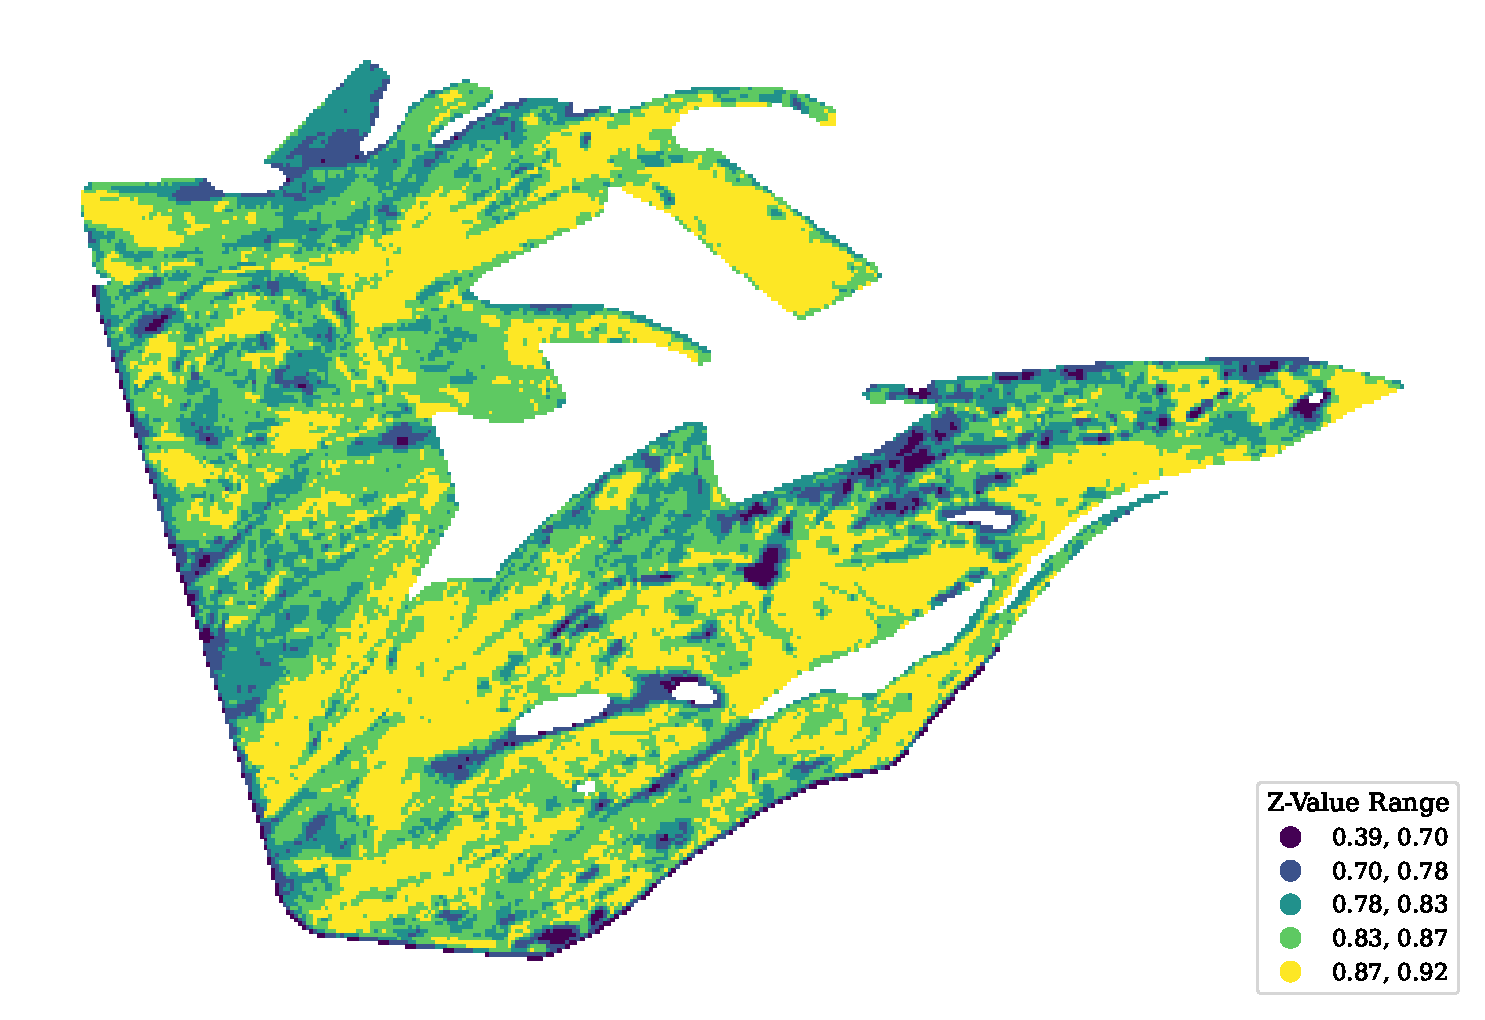
\includegraphics[width=\linewidth]{figures/original_Z_visualization.pdf}
            \caption{\scriptsize Productivity Distribution ($Z$)}
        \end{subfigure}
        \begin{subfigure}[b]{0.35\textwidth}
            \centering
            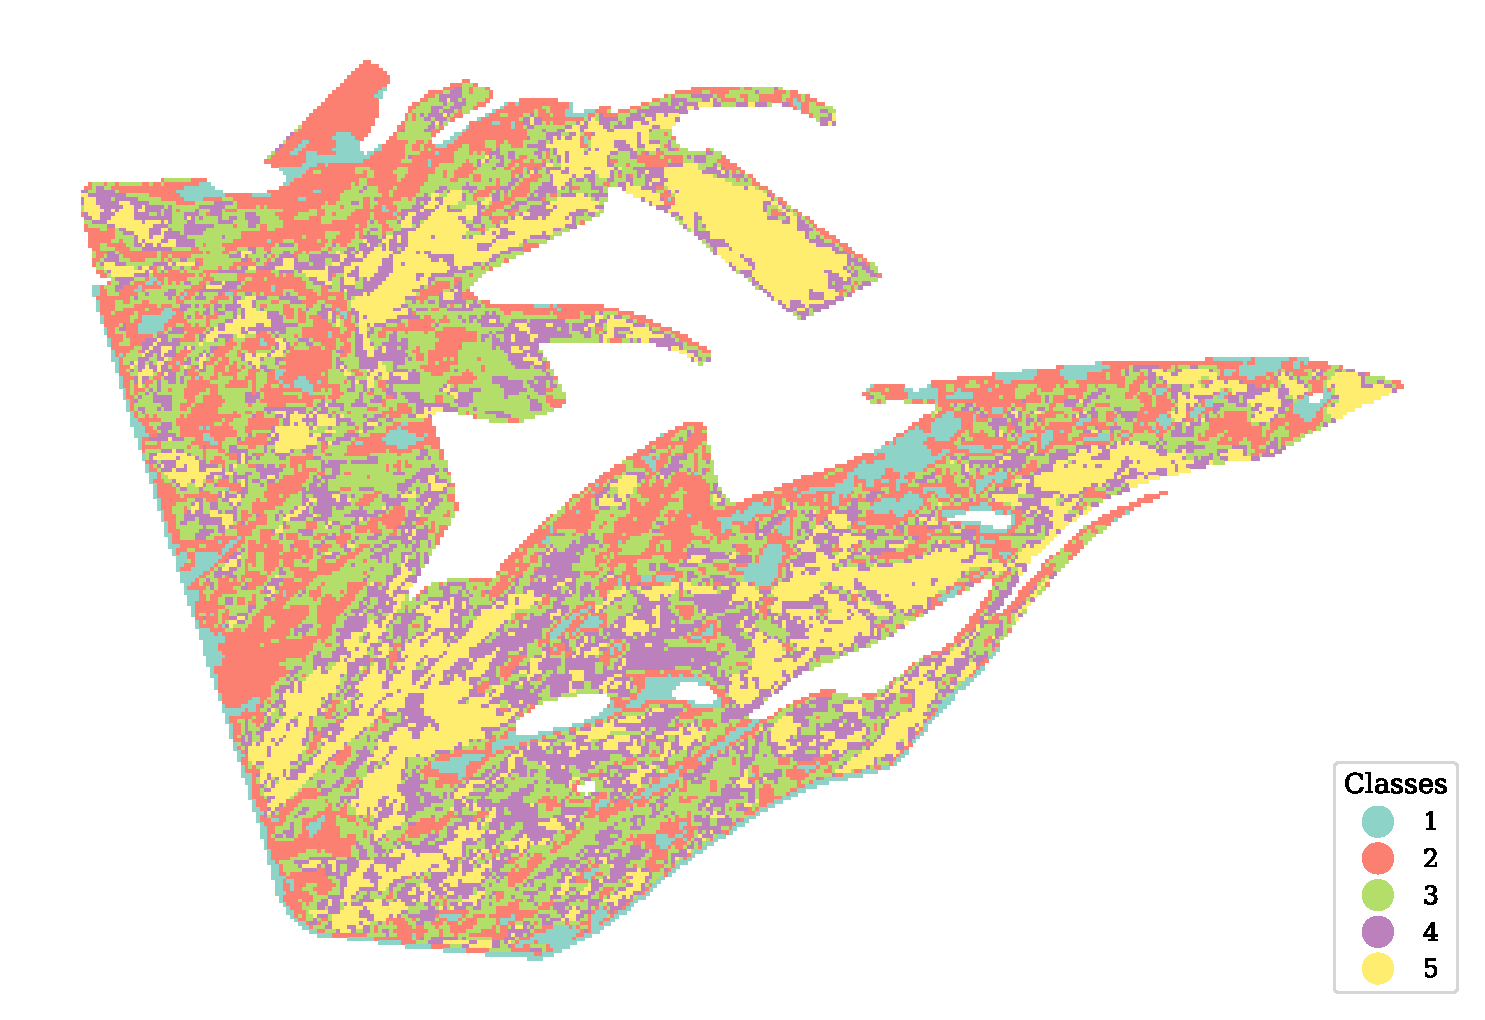
\includegraphics[width=\linewidth]{figures/original_label_visualization.pdf}
            \caption{\scriptsize Fragmented Categorical Map ($L$)}
        \end{subfigure}
    \end{figure}
    Here, the continuous physical attribute $Z$ represents a real-valued scalar
    corresponding to the maximum seasonal NDVI, and the categorical $L$ represents agricultural productivity levels.
    \begin{itemize}
        \item The continuous physical field (a) initially shows spatial autocorrelation.
        \item The categorical map (b) shows high-frequency noise.
    \end{itemize}
\end{frame}

% ================= PAGE 8 =================
\begin{frame}{Verification of Prerequisite: Spatial Autocorrelation}
    \begin{block}{Fundamental Assumption}
        Ordinary Kriging requires the attribute field $Z(\mathbf{X})$ to show spatial autocorrelation, rather than complete spatial randomness \cite{cressie2015statistics}.
    \end{block}

    \vspace{0.3cm}
    \begin{block}{Quantitative Assessment (Global Moran's I)}
        \begin{equation}
            I = \frac{N}{W} \frac{\sum_{i} \sum_{j} w_{ij}(Z_i - \bar{Z})(Z_j - \bar{Z})}{\sum_{i} (Z_i - \bar{Z})^2}
        \end{equation}
    \end{block}

    \begin{itemize}
        \item \textbf{Result:} A highly significant positive spatial autocorrelation ($I = 0.8002$, $p < 0.001$).
        \item \textbf{Implication:} This provides the theoretical support to model the physical field $Z(\mathbf{X})$ as a \textbf{Spatial Random Field (SRF)} and apply Kriging methods.
    \end{itemize}

\end{frame}

% ================= PAGE 9 =================
\begin{frame}{Data Normalization}
    \begin{columns}[T]
        \column{0.5\textwidth} % 稍微加宽左侧以容纳公式
        \textbf{Normality Violation:}
        Original data is apparently non-Normal distributed. This violates the normality assumption in later hypothesis testing, which will lead to biased predictions and invalid hypothesis testing \cite{wackernagel2003multivariate}.

        \textbf{Normal Score Transformation (NST)}
        \begin{equation}
            Y(\mathbf{X}_i) = \Phi^{-1}(F(Z(\mathbf{X}_i)))
        \end{equation}
        {\color{gray}\scriptsize \textit{* $\Phi^{-1}$: Inverse standard normal CDF; $F$: Cumulative Distribution Function of $Z$.}}

        \textbf{Transformation Results:}
        \begin{itemize}
            \item Regularized spatial skewness to $\approx 0$.
            \item The empirical quantiles align with the Gaussian diagonal (see Q-Q plot).
        \end{itemize}

        \column{0.48\textwidth}
        \begin{figure}
            \begin{subfigure}[b]{0.9\linewidth}
                \centering
                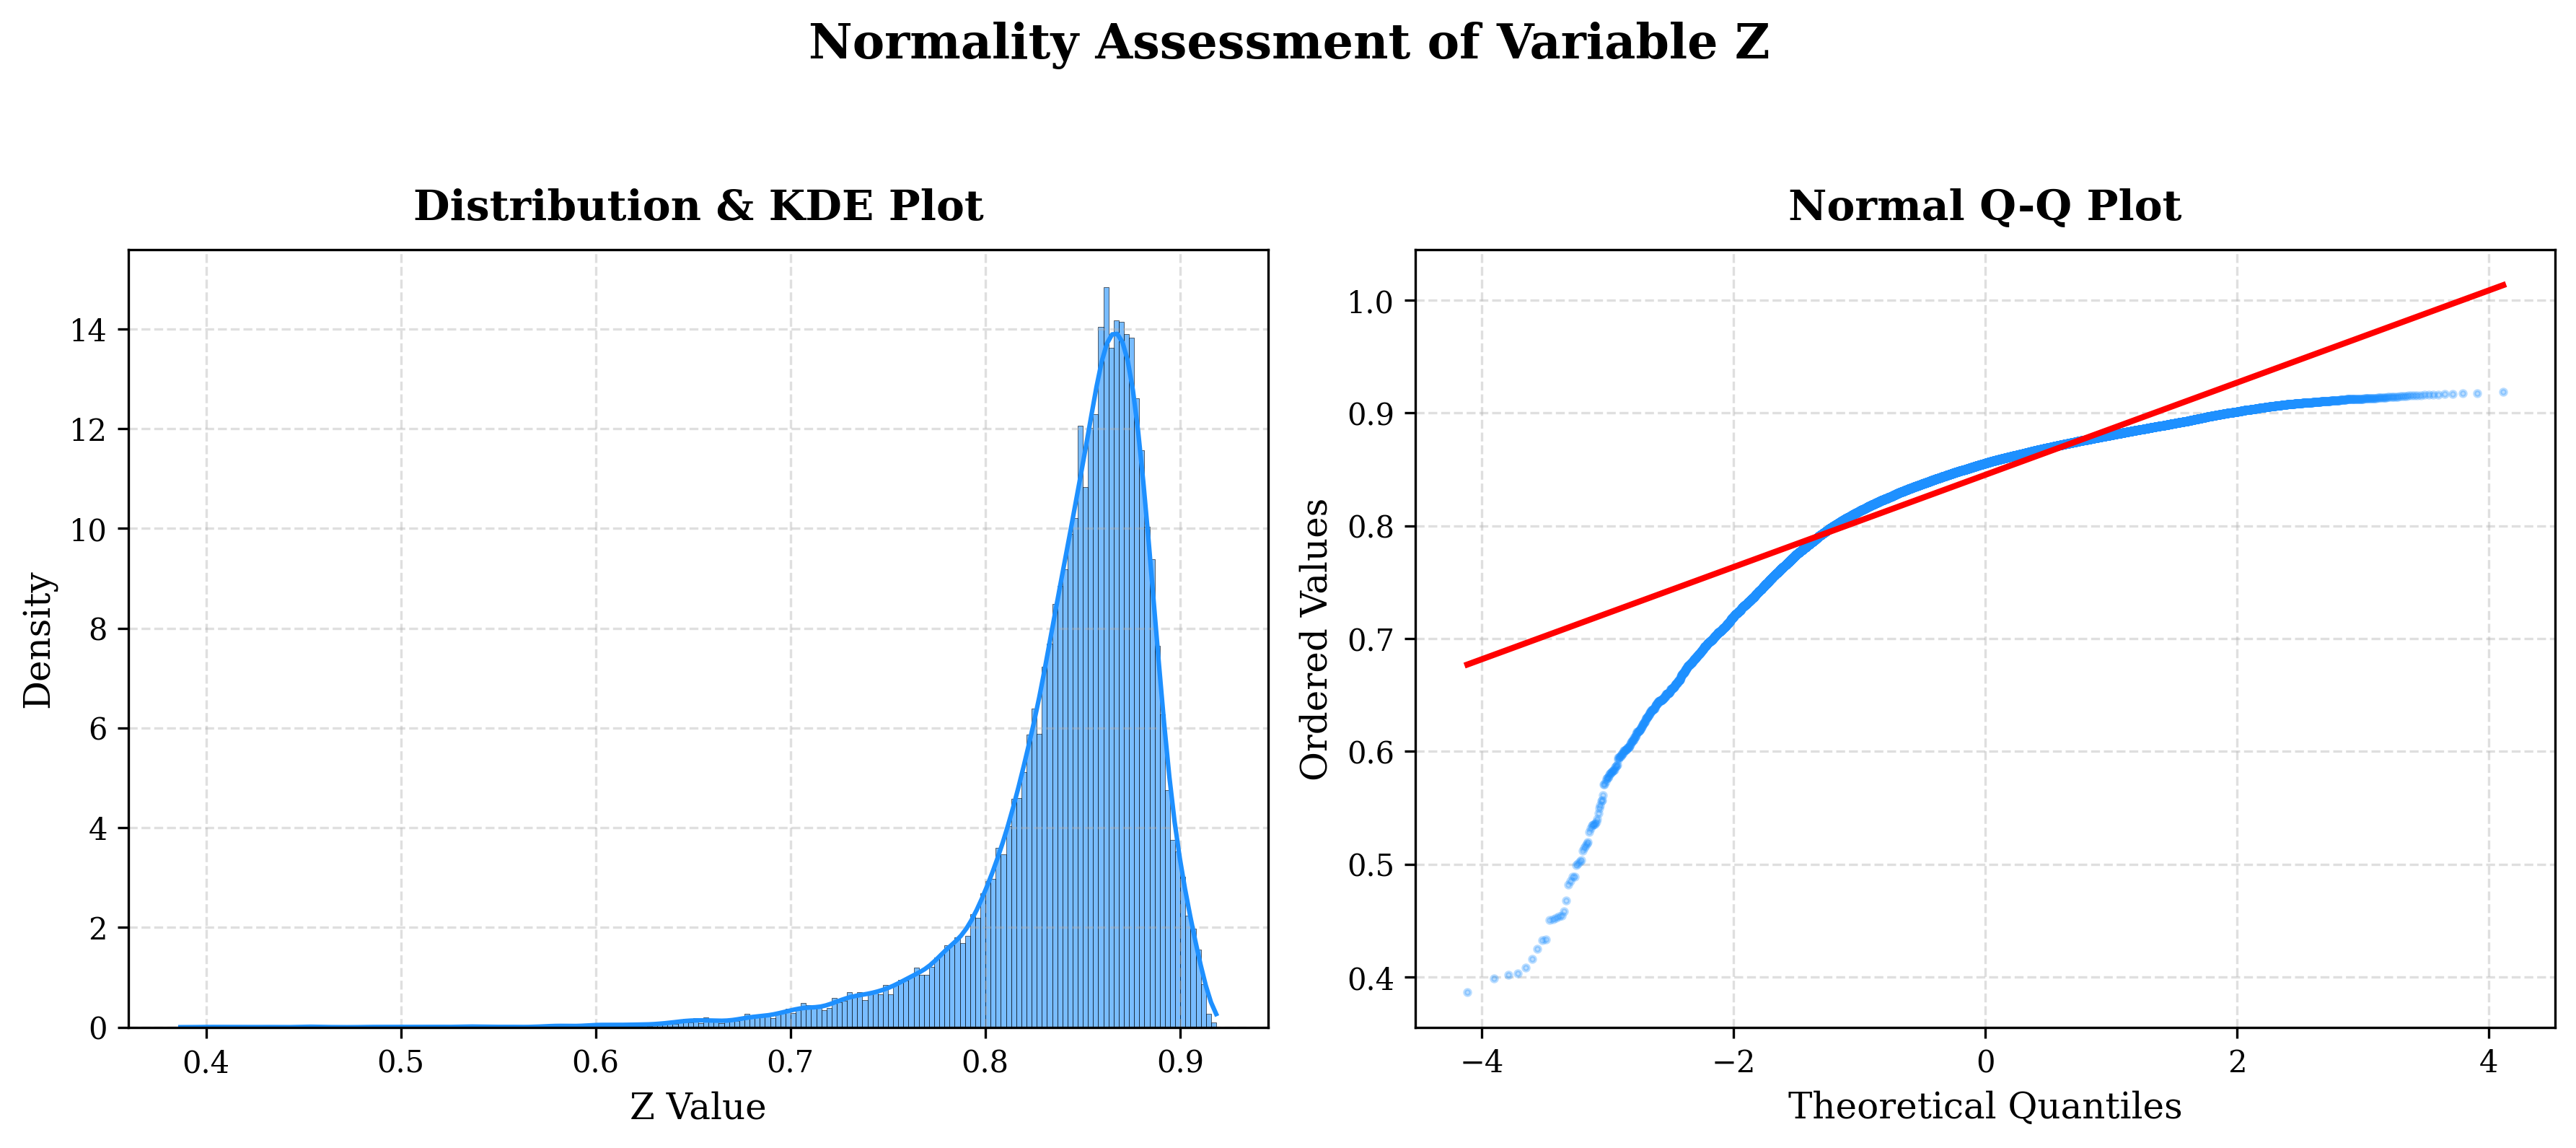
\includegraphics[width=\linewidth, keepaspectratio]{figures/Original His and QQ.png}
                \caption{\scriptsize Original $Z$ Histogram \& Q-Q Plot}
            \end{subfigure}
            \\
            \begin{subfigure}[b]{0.9\linewidth}
                \centering
                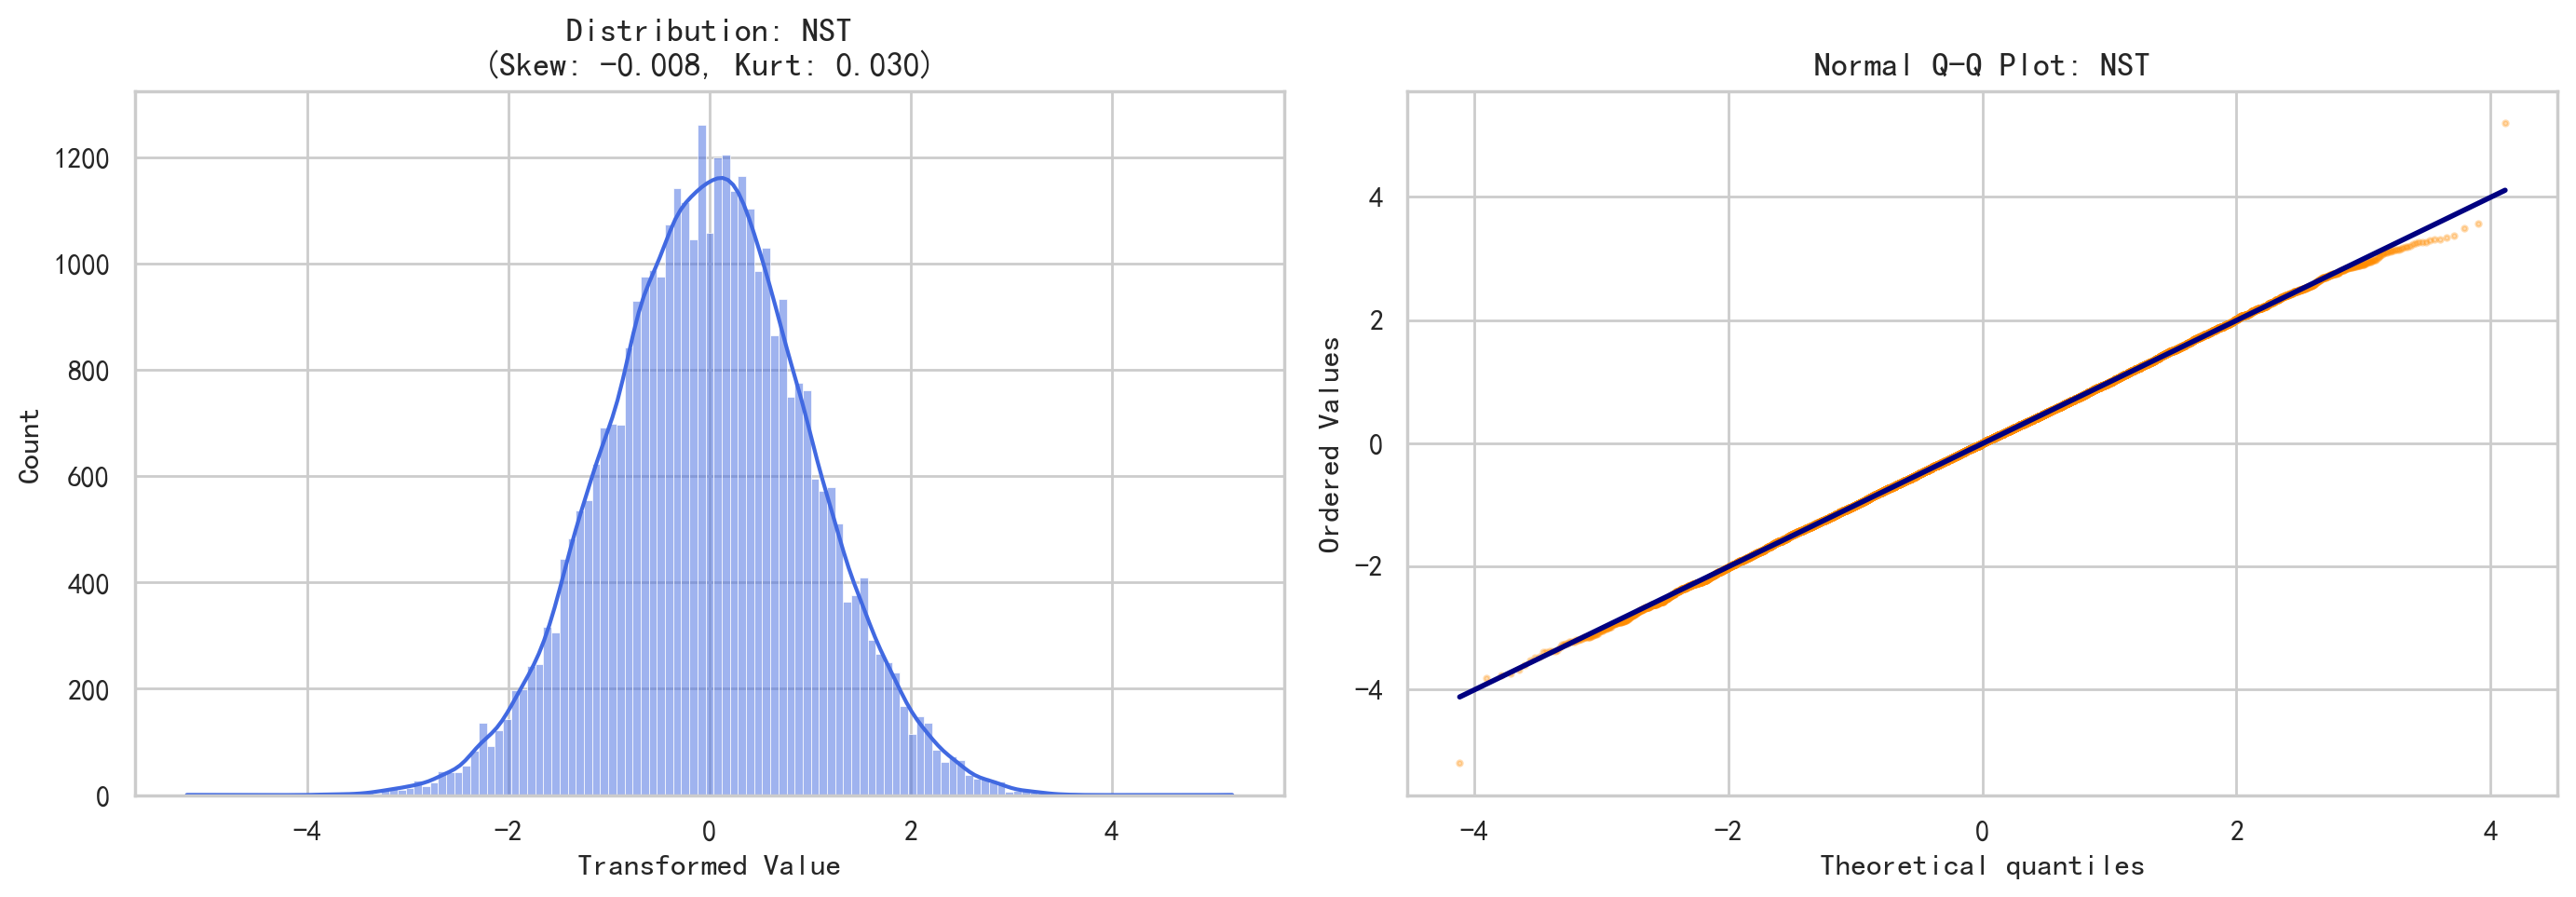
\includegraphics[width=\linewidth, keepaspectratio]{figures/Trans_Result_NST.png}
                \caption{\scriptsize NST Transformed $Y$ Histogram \& Q-Q Plot}
            \end{subfigure}
        \end{figure}
    \end{columns}
\end{frame}

% ==========================================
% 第三部分：方法论细节
% ==========================================
% 同样去除了硬编码的数字
\section{Methodology: Geostatistical Refinement Pipeline}

% ================= PAGE 10 =================
\begin{frame}{Step 1: Isolation Detection (Candidate Extraction)}
    \textbf{Objective:} Identify spatially isolated pixels, which are likely misclassified rather than being true geographical features.

    \begin{block}{Mathematical Metrics}
        \begin{itemize}
            \item \textbf{Neighbor Disagreement Score (NDS):} Measures spatial mismatch.
                  \begin{equation}
                      NDS(\mathbf{X}_i) = \frac{1}{|\mathcal{N}_i|} \sum_{j \in \mathcal{N}_i} \mathbb{I}\Big(L(\mathbf{X}_j) \neq L(\mathbf{X}_i)\Big)
                  \end{equation}
                  \textit{* $\mathbb{I}(\cdot)$ is the indicator function; $\mathcal{N}_i$ defines the Moore neighborhood.}

            \item \textbf{Connected Components Analysis (CCA):} Evaluates spatial connectivity to flag clusters below the set Minimum Unit.
        \end{itemize}
    \end{block}


    \textbf{Algorithmic Logic:}
    Denote $\mathcal{S}$ as the set of all pixels, $\mathcal{S}_{\text{NDS}}$ as the set of pixels with $NDS > \tau$ (e.g., $\tau=0.8$), and $\mathcal{S}_{\text{CCA}}$ as the set of pixels in connected components smaller than the Minimum Unit (e.g., 4 pixels).
    The pixels within the union set $\mathcal{S}_{\text{cand}} = \mathcal{S}_{\text{NDS}} \cup \mathcal{S}_{\text{CCA}}$ are considered isolated and serve as prediction targets in the subsequent Kriging stage.
\end{frame}

% ================= PAGE 11 =================
\begin{frame}{Step 2: Geostatistical Validation (Ordinary Kriging)}
    For candidate $\mathbf{X}_0 \in \mathcal{S}_{\text{cand}}$, we use Ordinary Kriging to predict the expected value $\hat{Z}(\mathbf{X}_0)$ and measure the associated uncertainty $\sigma^2_K(\mathbf{X}_0)$.
    \begin{block}{Kriging Methodology}
        \begin{align}
            \textbf{Estimator: } \hat{Z}(\mathbf{X}_0)   & = \sum_{i=1}^{n} \lambda_i Z(\mathbf{X}_i), \quad \mathbf{X_i} \in \mathcal{S}_{\text{reference}} = \mathcal{S} \backslash \mathcal{S}_{\text{cand}}   \\
            \textbf{Variance: } \sigma^2_K(\mathbf{X}_0) & = 2 \sum_{i=1}^{n} \lambda_i \gamma(\mathbf{X}_i, \mathbf{X}_0) - \sum_{i=1}^{n} \sum_{j=1}^{n} \lambda_i \lambda_j \gamma(\mathbf{X}_i, \mathbf{X}_j)
        \end{align}
        $\lambda_i$ are the Kriging weights determined by solving the Kriging system of equations, $\gamma$ is the semivariogram to model spatial dependence.
    \end{block}

    \begin{columns}[T]
        \column{0.48\textwidth}
        \textbf{Why Ordinary Kriging?}
        \begin{itemize}
            \item Best Linear Unbiased Predictor.
            \item Provides \alert{physically grounded uncertainty} $\sigma^2_K$.
        \end{itemize}

        \column{0.48\textwidth}
        \textbf{Computational Optimization:}
        The computation complexity is \alert{$\mathcal{O}(N^3)$}, therefore uses only reference pixels that are within a certain distance from the candidate pixel.
    \end{columns}
\end{frame}

% ================= PAGE 12 =================
\begin{frame}{Step 3: Hypothesis Testing Framework}
    \begin{itemize}
        \item \textbf{$H_0$ (The "Normal" case):} The observed value at this location is consistent with the surrounding area. {\color{gray} It looks like something that would naturally occur given its neighbors.}
        \item \textbf{$H_A$ (The "Outlier" case):} The observed value is out of place. {\color{gray} It seems to come from a different process, meaning it doesn't fit in with the nearby environment.}
    \end{itemize}

    \vspace{0.2cm}
    \textbf{Test Statistic $\eta(\mathbf{X}_0)$:}
    \begin{equation}
        \eta(\mathbf{X}_0) = \frac{Z_{\text{obs}}(\mathbf{X}_0) - \hat{Z}(\mathbf{X}_0)}{\sigma(\mathbf{X}_0)} \sim \mathcal{N}(0,1)
    \end{equation}
    {\centering \color{gray}\scriptsize \textit{* Asymptotic normality is mathematically guaranteed by the prior NST step.}\\ \par}

    To avoid the multiple testing problem across all candidates, we apply the Benjamini-Hochberg procedure to control the False Discovery Rate (FDR) at a pre-specified level $q=0.05$.

    \begin{block}{Decision Rule}
        \begin{enumerate}
            \item \textbf{Reject $H_0$:} Large physical difference $\to$ \textbf{Keep original label} (Real feature).
            \item \textbf{Fail to reject $H_0$:} Small difference $\to$ \textbf{Proceed to Reassignment} (Noise).
        \end{enumerate}
    \end{block}
\end{frame}

% ================= PAGE 13 =================
\begin{frame}{Step 4: Likelihood-Based Class Reassignment}
    \begin{block}{Kriging-Based Likelihood Function}
        For each candidate class $C_k \in \mathcal{C}$, we compute the likelihood of observing $Z_{\text{obs}}(\mathbf{X}_0)$:
        \begin{equation}
            \mathcal{L}(C_k, \mathbf{X}_0) = \frac{1}{\sigma_{C_k}(\mathbf{X}_0)} \exp \left( - \frac{(Z_{\text{obs}}(\mathbf{X}_0) - \hat{Z}_{C_k}(\mathbf{X}_0))^2}{2\sigma^2_{C_k}(\mathbf{X}_0)} \right)
        \end{equation}
        \textit{* $\hat{Z}_{C_k}(\mathbf{X}_0)$ and $\sigma^2_{C_k}(\mathbf{X}_0)$ are the Kriging prediction and variance computed using only the reference pixels belonging to class $C_k$, i.e., $\mathcal{S}_{\text{ref}}(C_k) = \{ \mathbf{X}_i : L(\mathbf{X}_i) = C_k \}$.}
    \end{block}

    \vspace{0.2cm}
    \begin{itemize}
        \item \textbf{Structural Regularization:} The leading term $\sigma^{-1}_{C_k}$ mathematically penalizes candidate classes that show high spatial uncertainty or limited local data.
        \item The corrected final label $L^*$ is chosen to maximize the likelihood function across all candidate classes $\mathcal{C}$ (i.e., all 5 classes):
              \begin{equation*}
                  L^*(\mathbf{X}_0) = \underset{C_k \in \mathcal{C}}{\arg\max} \,\, \mathcal{L}(C_k, \mathbf{X}_0)
              \end{equation*}
    \end{itemize}

\end{frame}

% ==========================================
% 第四部分：实验结果分析
% ==========================================
\section{Results and Analysis}

% ================= PAGE 14 =================
\begin{frame}{Result 1: Extraction of Candidate Outliers}

    \begin{figure}
        \centering
        \begin{subfigure}[b]{0.35\linewidth}
            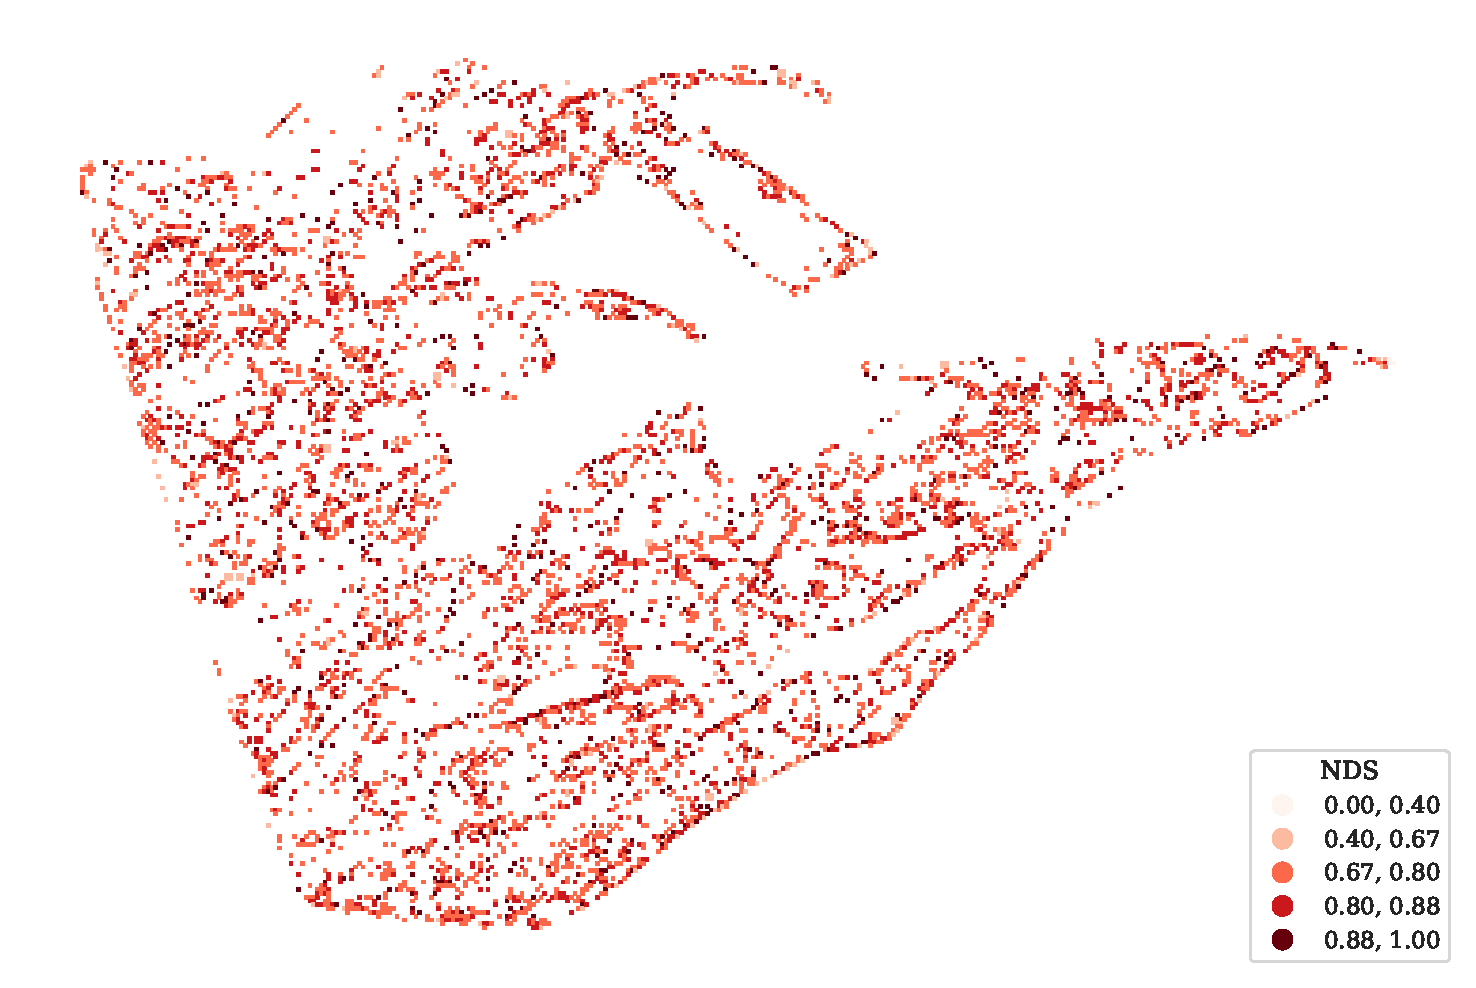
\includegraphics[width=\linewidth, keepaspectratio]{figures/isolatations_NDS_visualization_map.pdf}
            \caption{Continuous NDS Distribution}
        \end{subfigure}
        \begin{subfigure}[b]{0.35\linewidth}
            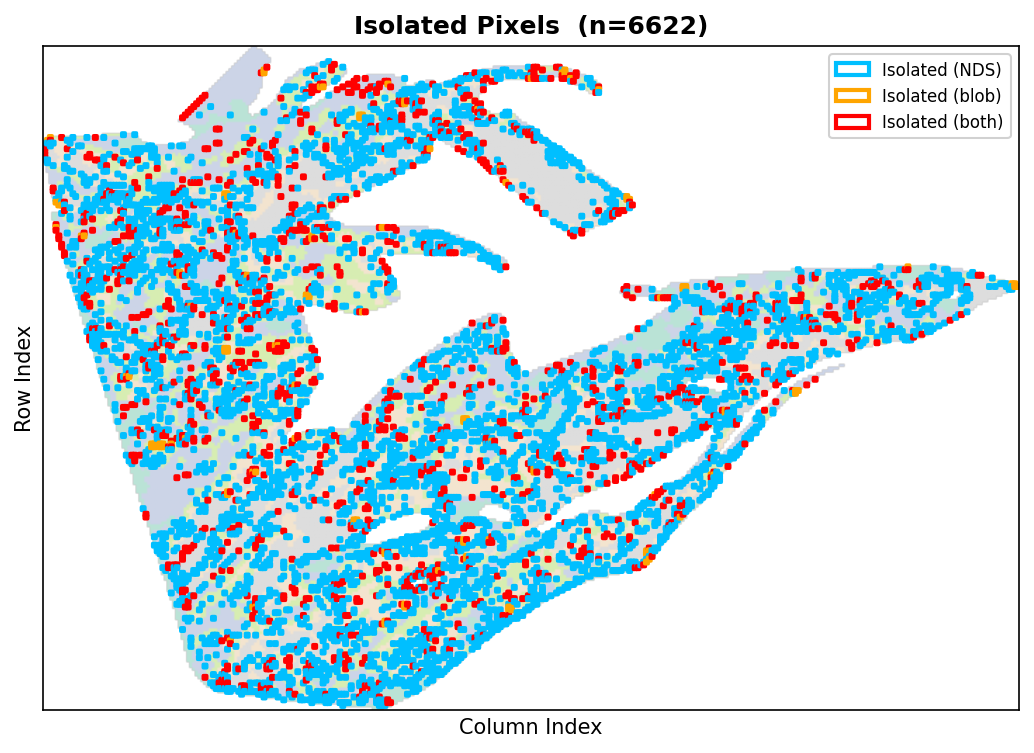
\includegraphics[width=\linewidth, keepaspectratio]{figures/transed_data_isolation_3_isolated.png}
            \caption{Extracted Spatial Candidates}
        \end{subfigure}
    \end{figure}
    \textbf{Observations from Step 1:}
    \begin{itemize}
        \item \textbf{NDS Map (a):} High spatial mismatches are primarily clustered along class boundaries.
        \item \textbf{Candidates (b):} Effectively isolates the "salt-and-pepper" noise patches. \textbf{6,622 pixels} flagged as candidates ($\approx 18.4\%$ of total domain).
    \end{itemize}

\end{frame}

% ================= PAGE 15 =================
\begin{frame}{Result 2: Semivariogram Modeling}
    Based on the weighted Root Mean Square Error (wRMSE), the Exponential model demonstrated the most optimal fit.
    \begin{columns}[c]
        \column{0.6\textwidth}
        \begin{figure}
            \centering
            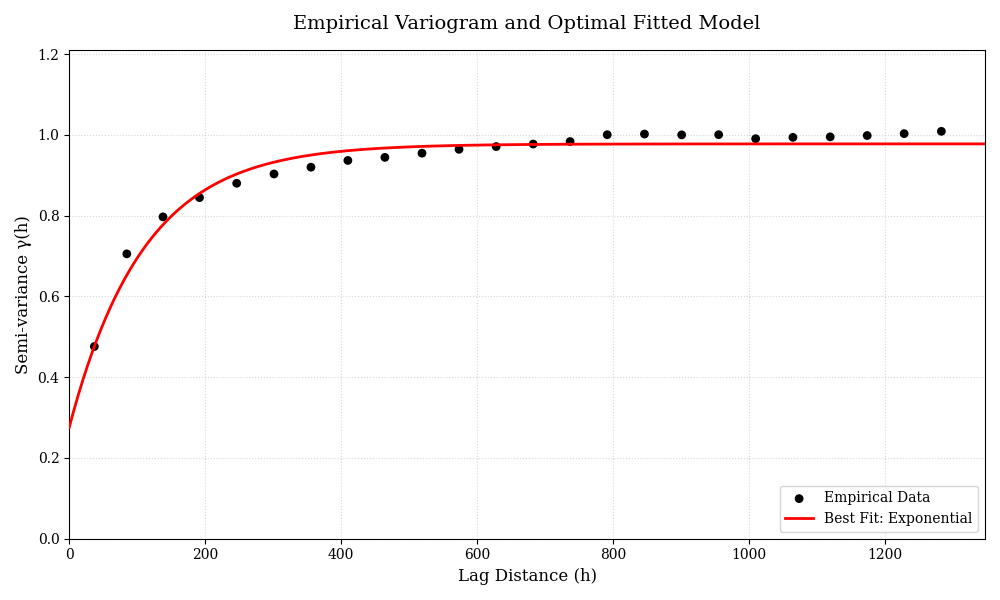
\includegraphics[width=0.9\linewidth, keepaspectratio]{figures/optimal_variogram_plot.png}
            \caption{\scriptsize Empirical Semivariogram (black dots) and Fitted Models: Exponential (red).}
        \end{figure}

        \column{0.35\textwidth}
        \textbf{Fitted Parameters:}
        \begin{itemize}
            \item \textbf{Nugget ($c_0$):} 0.275, reflects inherent sensor/environmental noise.
            \item \textbf{Sill ($c$):} 0.978, indicates the total variance of the spatial process.
            \item \textbf{Range ($a$):} 110.0 meters, defines the spatial correlation distance.
        \end{itemize}

    \end{columns}

\end{frame}

% ================= PAGE 16 =================
\begin{frame}{Result 3 \& 4: Kriging Validation \& Statistical Decisions}
    \begin{columns}
        \column{0.65\textwidth}
        \begin{figure}
            \begin{subfigure}[b]{0.48\linewidth}
                \centering
                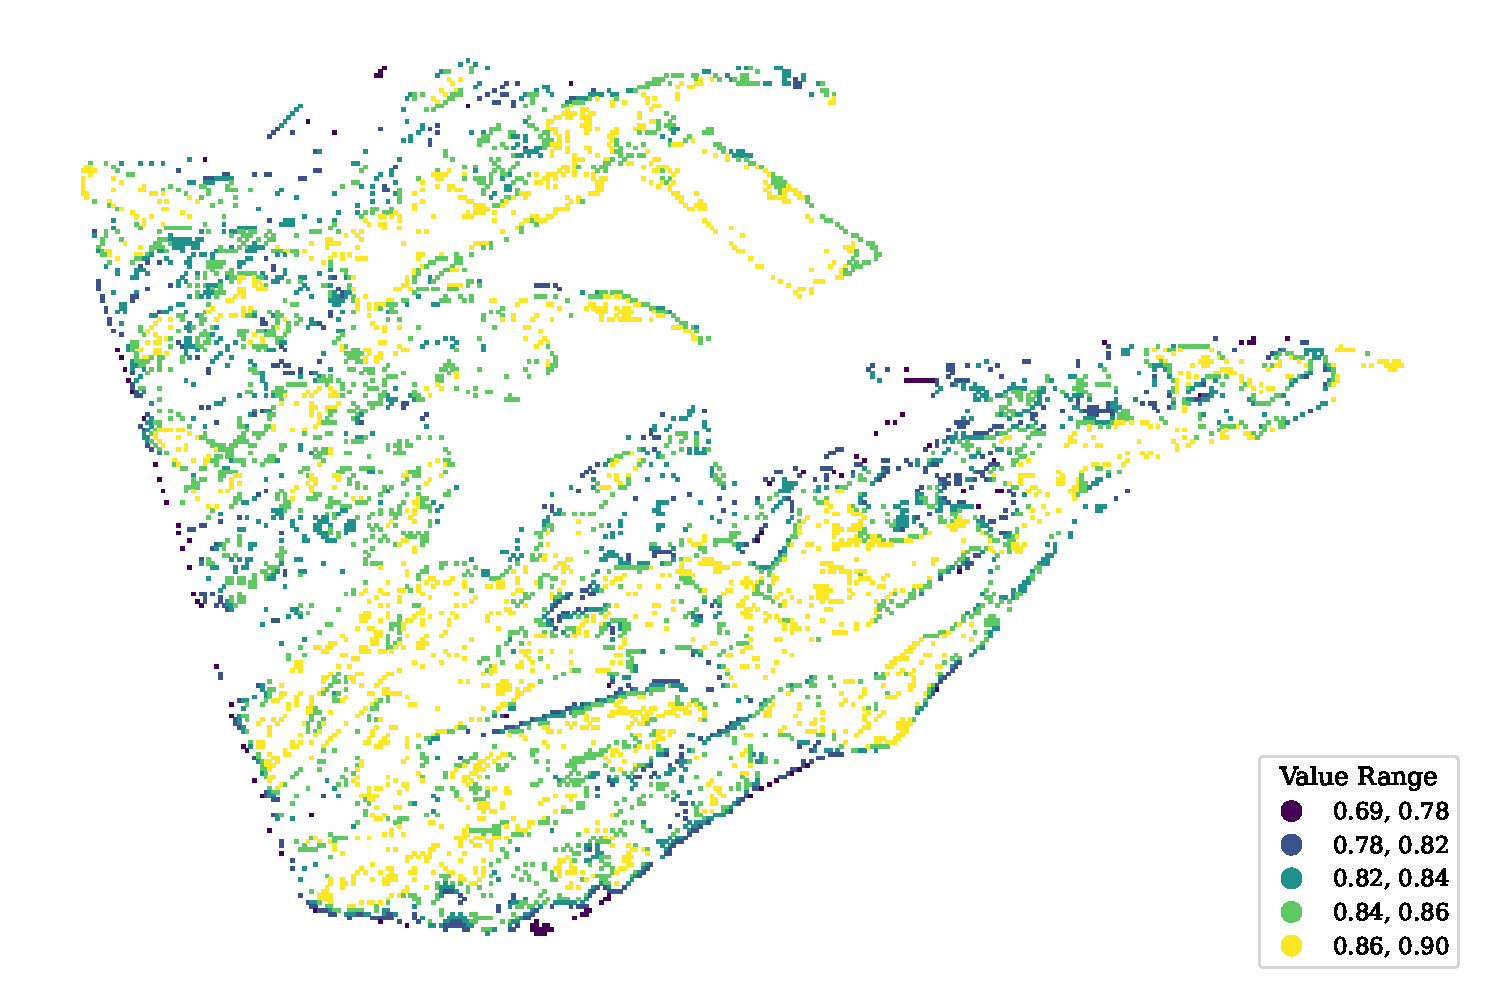
\includegraphics[width=\linewidth, keepaspectratio]{figures/kriged_Zback_visualization_map.pdf}
                \caption{\scriptsize Kriging Prediction Field ($\hat{Z}$)}
            \end{subfigure}
            \vspace{0.15cm}
            \begin{subfigure}[b]{0.48\linewidth}
                \centering
                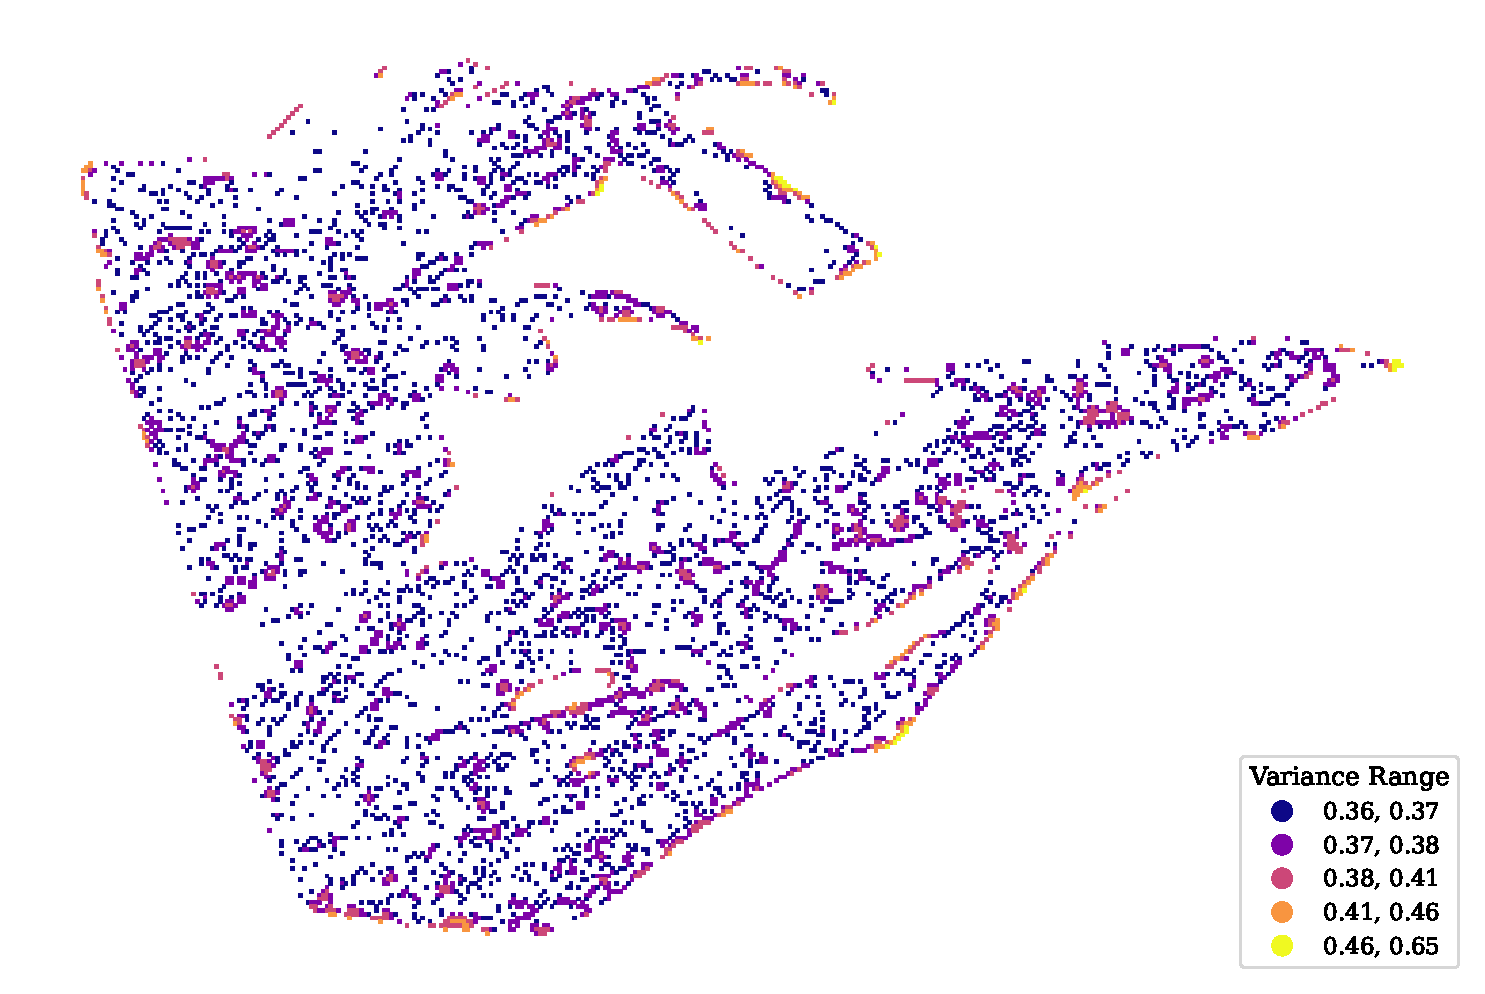
\includegraphics[width=\linewidth, keepaspectratio]{figures/kriged_variance_visualization_map.pdf}
                \caption{\scriptsize Kriging Variance Field ($\sigma^2_K$)}
            \end{subfigure}
        \end{figure}

        \column{0.33\textwidth}
        \begin{itemize}
            \item \textbf{Prediction (a):} Smooth continuous field behind categorical noise.
            \item \textbf{Variance (b):} Uncertainty spatially measured ($\sigma^2_K \in [0.36, 0.65]$); high variance zones guide hypothesis testing.
        \end{itemize}
    \end{columns}

    \begin{columns}
        \column{0.6\textwidth}
        \textbf{FDR Control at $q = 0.05$:}
        \begin{center}
            \renewcommand{\arraystretch}{1.2}
            \begin{tabular}{lcc}
                \toprule
                \textbf{Statistical Category}        & \textbf{Count}    & \textbf{percentage, \%} \\
                \midrule
                Total Candidates ($S_{\text{cand}}$) & 6,622             & 100\%                   \\
                \textbf{Rejected $H_0$}              & \textbf{6}        & \textbf{0.1\%}          \\
                \color{gray}Fail to reject $H_0$     & \color{gray}6,616 & \color{gray}99.9\%      \\
                \bottomrule
            \end{tabular}
        \end{center}

        \column{0.38\textwidth}
        \begin{itemize}
            \item 99.9\% of the "salt-and-pepper" noise considered as noise pixels.
            \item FDR test keeps \textbf{6 real micro-structures} that standard filters would have removed.
        \end{itemize}
    \end{columns}
\end{frame}

% ================= PAGE 19 =================
\begin{frame}{Result 5: Label Correction Analysis and Comparison}
    \begin{figure}
        \centering
        \begin{subfigure}[b]{0.3\linewidth}
            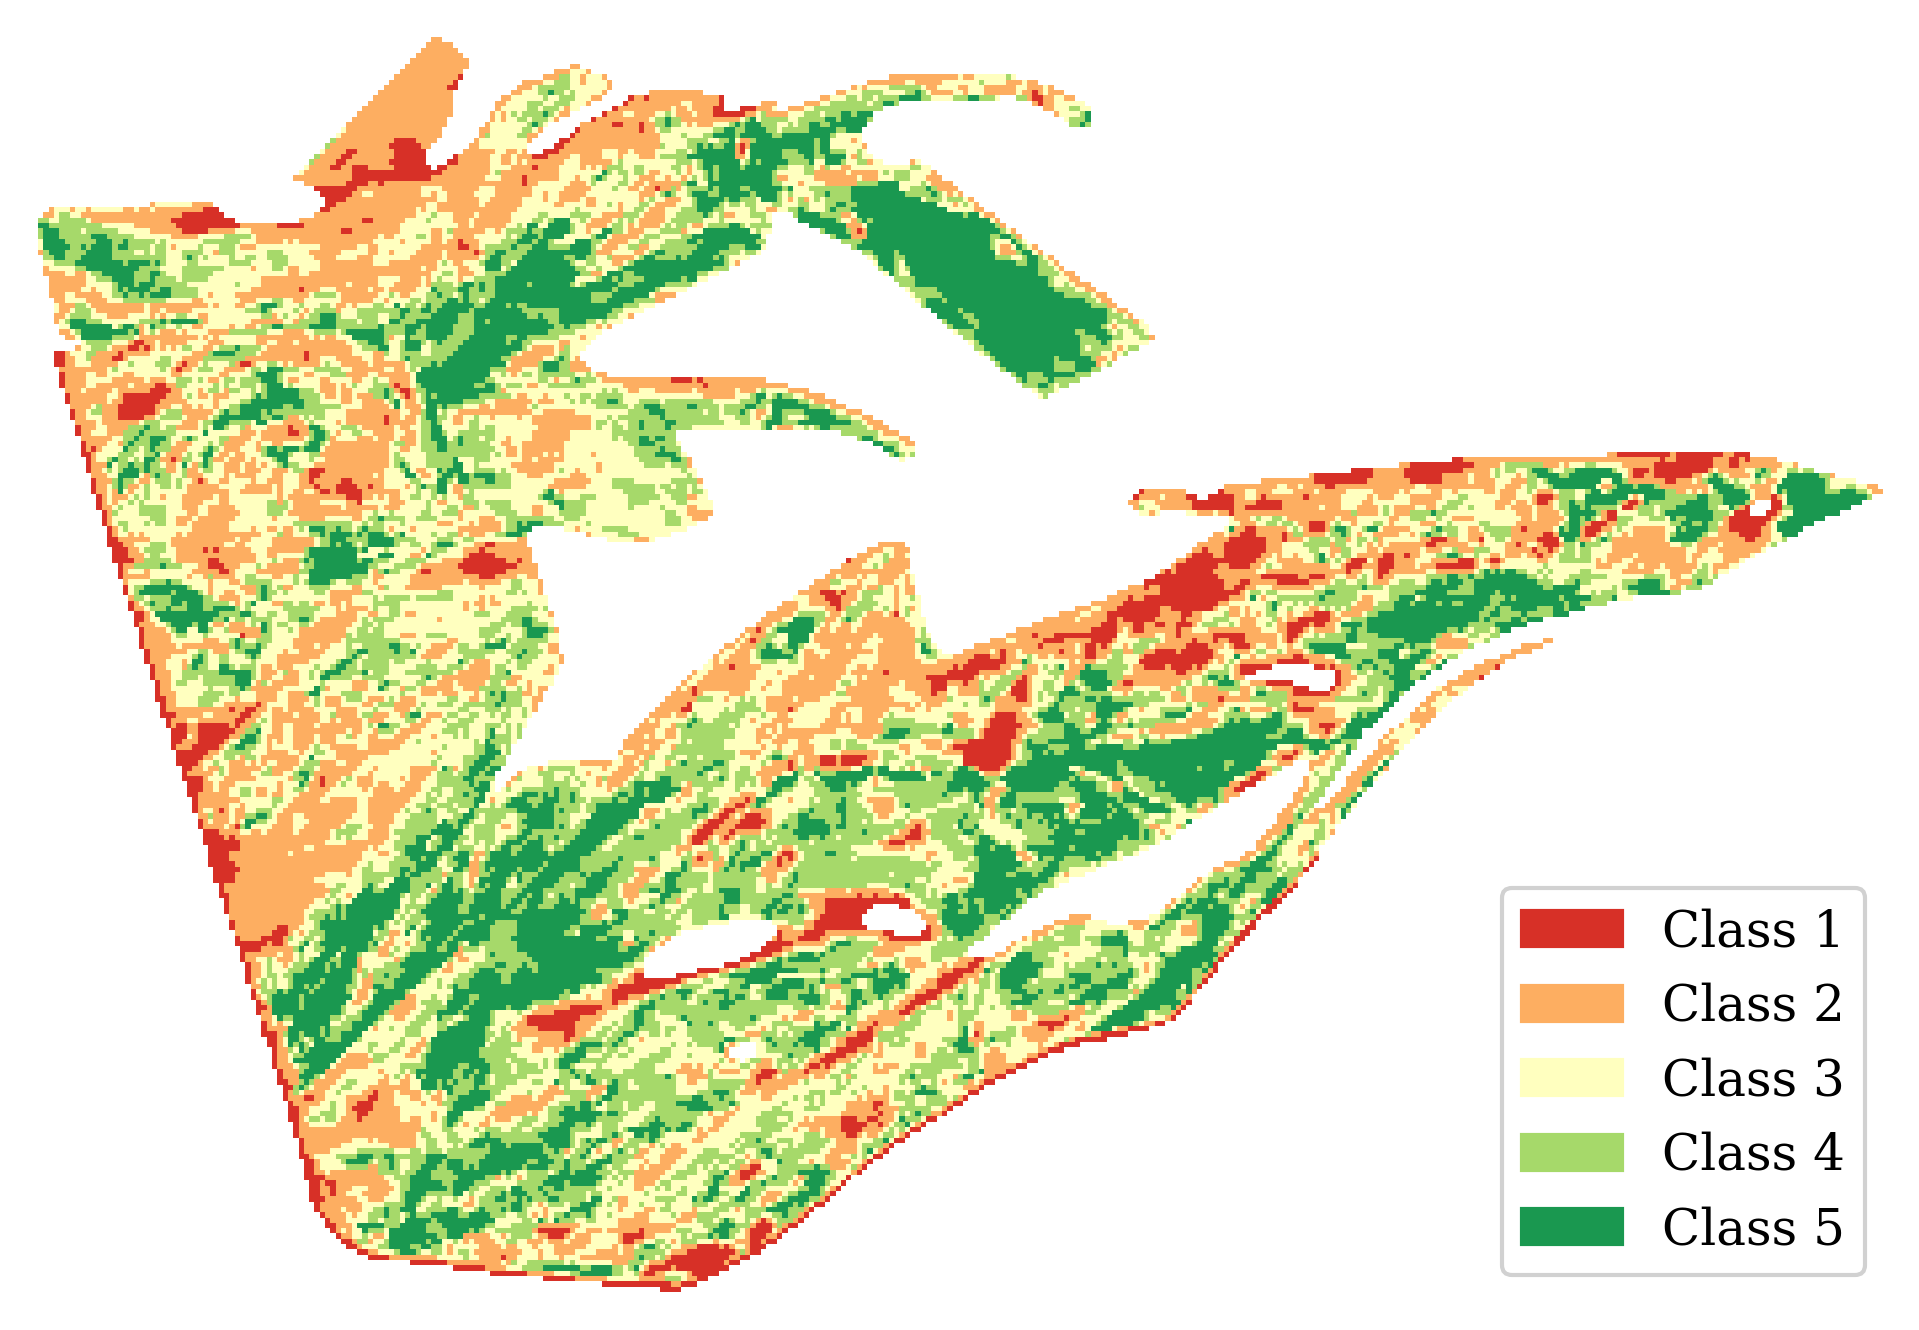
\includegraphics[width=\linewidth]{figures/thesis_single_a_original.png}
            \caption{\scriptsize Original Fragmented Map}
        \end{subfigure}
        \begin{subfigure}[b]{0.3\linewidth}
            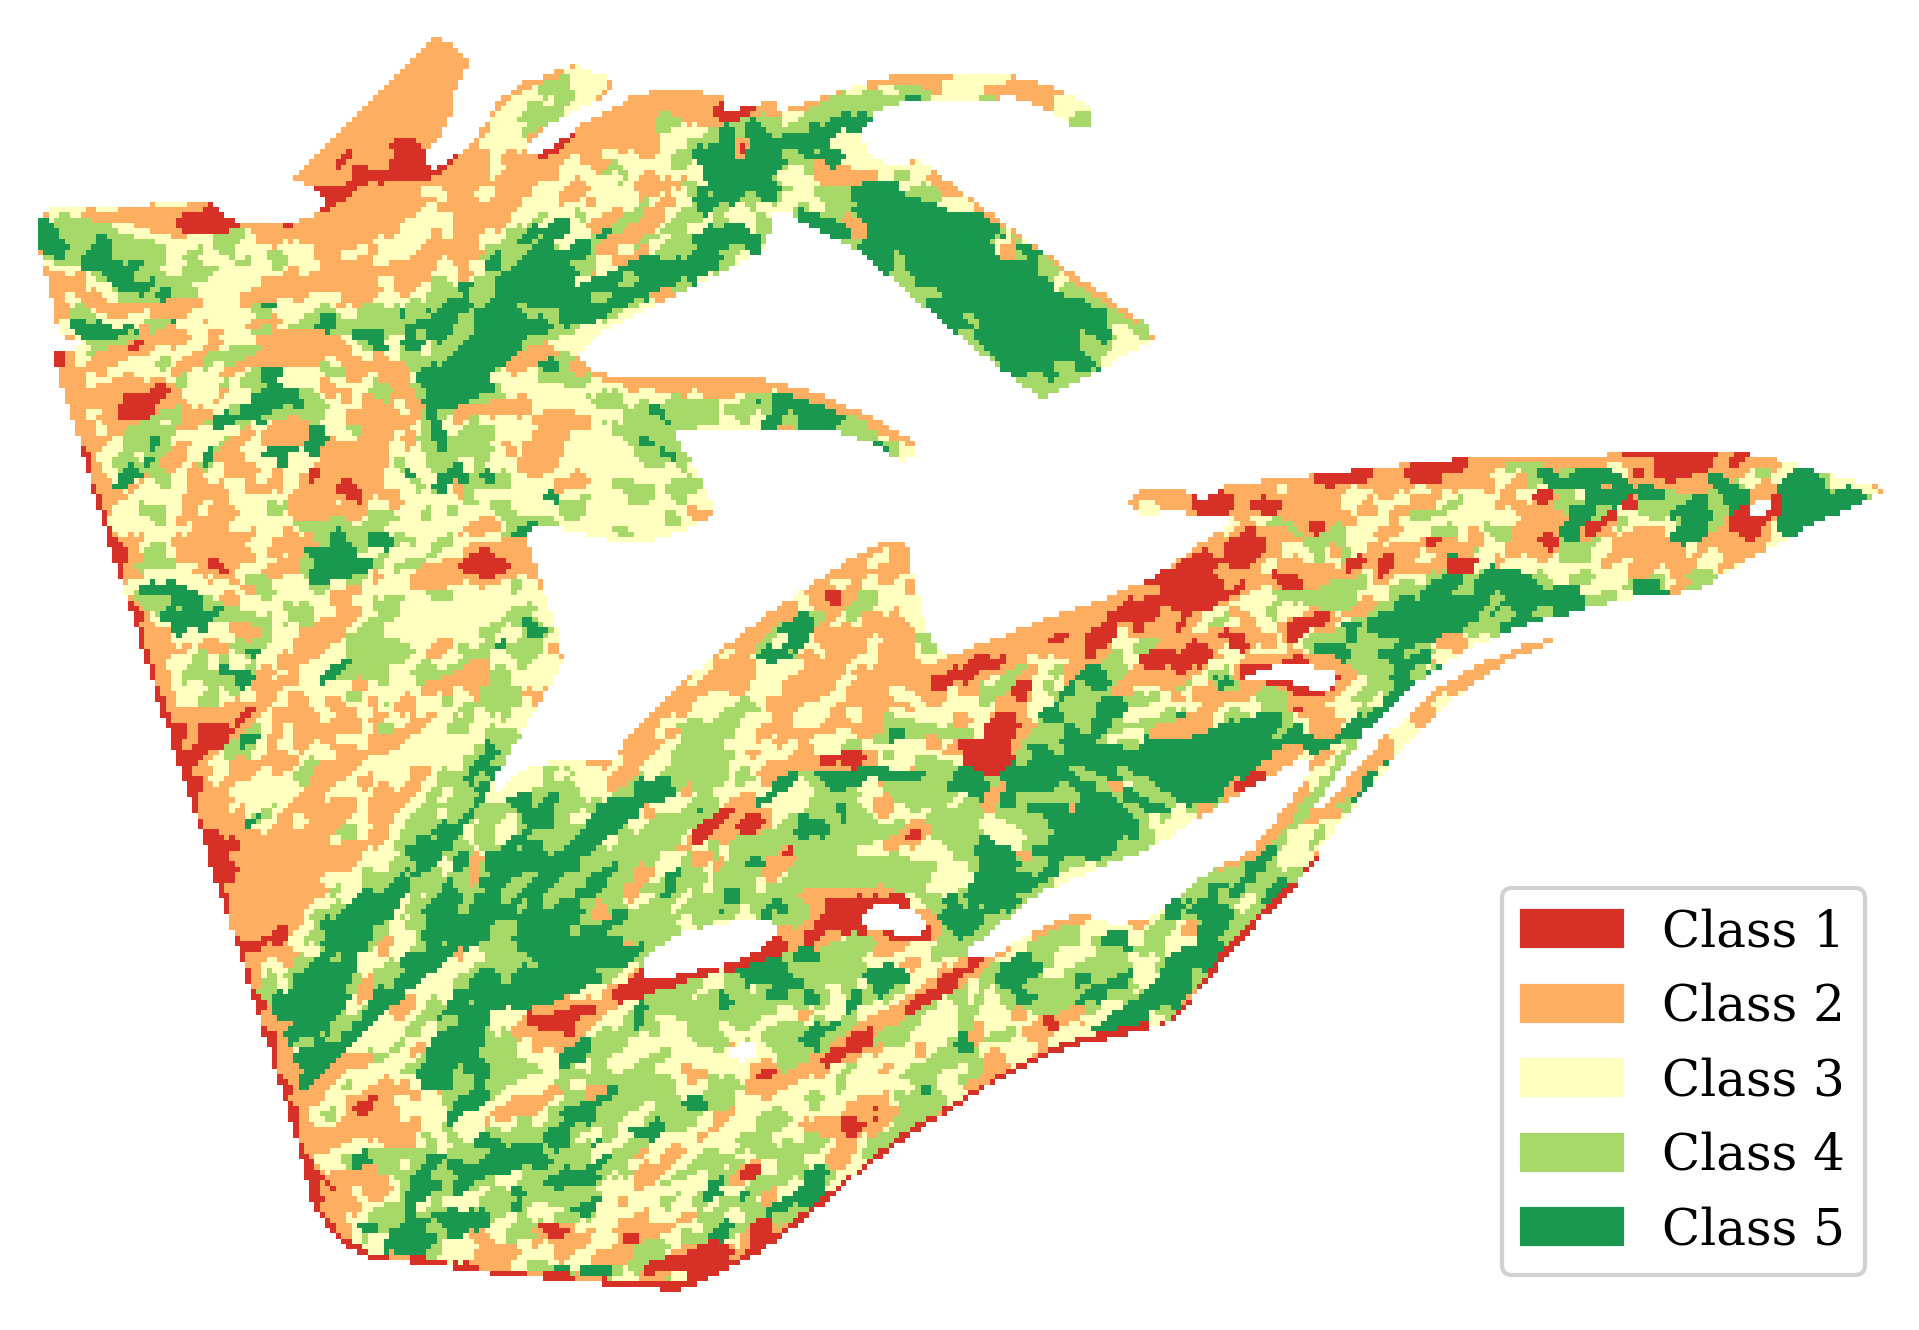
\includegraphics[width=\linewidth]{figures/thesis_single_b_refined.png}
            \caption{\scriptsize Refined Map}
        \end{subfigure}
        \begin{subfigure}[b]{0.3\linewidth}
            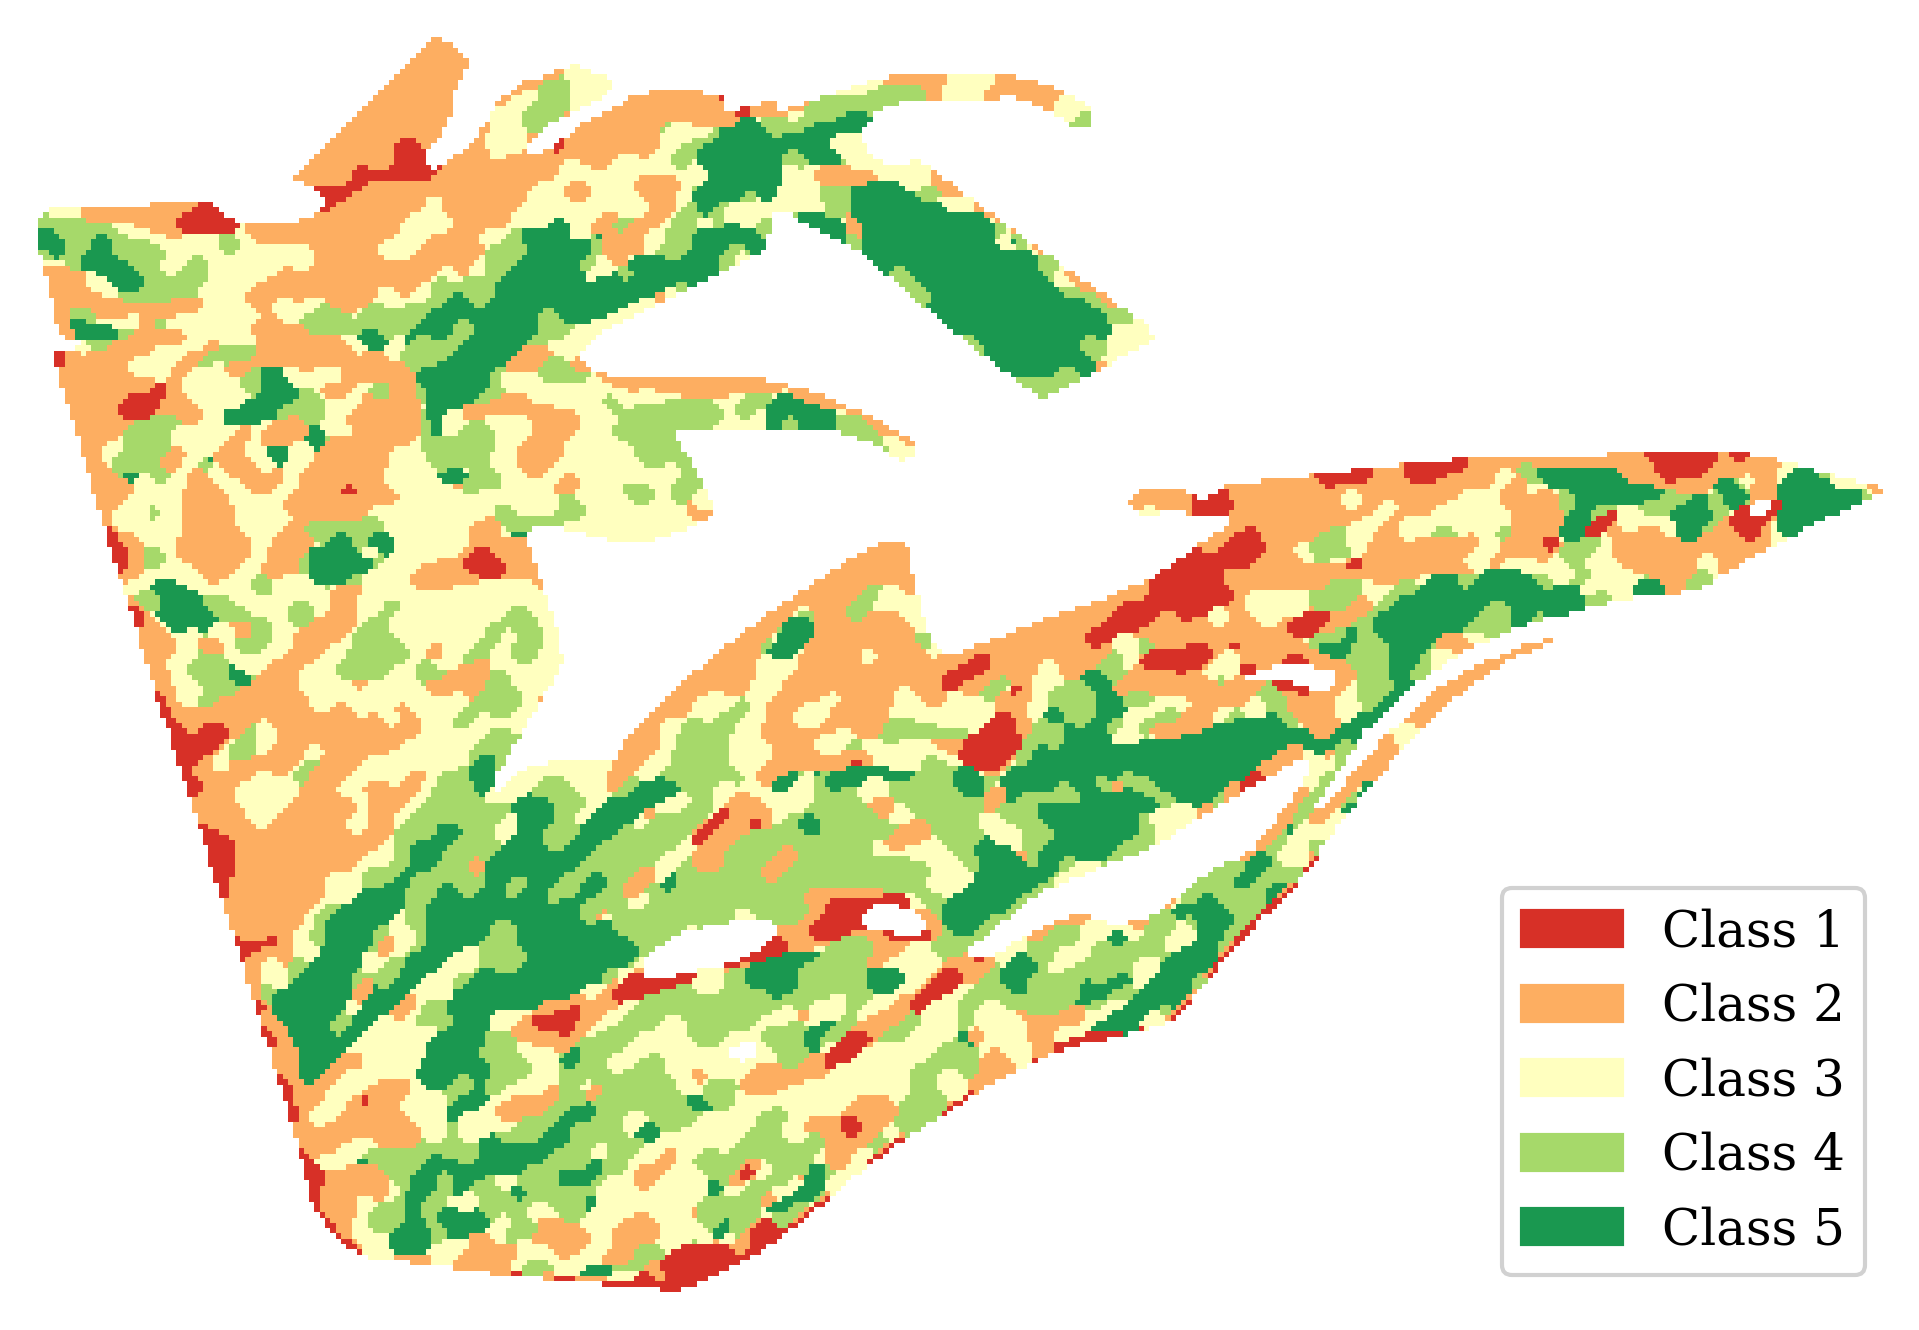
\includegraphics[width=\linewidth]{figures/filtered_single_b_refined.png}
            \caption{\scriptsize Majority Filtered Map}
        \end{subfigure}
    \end{figure}

    \begin{itemize}
        \item The Kriging-based refinement (b) reassigns 5,180 pixels, retaining 1,436 pixels, which are original micro-features. It is a blance between noise removal and feature preservation.
        \item In contrast, the Majority Filter (c) reassigns 9,542 pixels and over-smooths the map.
    \end{itemize}
\end{frame}

% ==========================================
% 第五部分：总结与展望
% ==========================================
\section{Conclusion}

% --- 第 21 页：结论与未来展望 (Conclusion & Future Work) ---
\begin{frame}{Conclusion \& Future Directions}
    \textbf{Research Summary:}
    \begin{itemize}
        \item Transitioned post-classification from "geometric cleanup" to \textbf{formal spatial inference}.
        \item Successfully balanced strong noise removal with the keeping of micro-scale geographic realities.
    \end{itemize}

    \vspace{0.3cm}
    \textbf{Future Research Directions:}
    \begin{itemize}
        \item Replace OK with \textbf{Universal Kriging} or \textbf{Regression Kriging} to include additional variables (e.g., DEM, Soil Moisture).
        \item Expanding $\gamma(\mathbf{h})$ into \textbf{3D semivariograms} $\gamma(\mathbf{h}, t)$ to validate pixels against their historical physical paths.
        \item Using cross-correlation between multiple spectral indices to improve refinement stability.
    \end{itemize}
\end{frame}

% --- 参考文献页 ---
% 使用 allowframebreaks 自动处理多页参考文献
\begin{frame}[allowframebreaks]{References}
    \printbibliography[heading=none]
\end{frame}

% ================= PAGE 23 =================
\begin{frame}[plain] % plain 隐藏掉页脚和导航栏，让致谢页更纯粹
    \centering
    \vspace{1.5cm}
    {\Huge \textbf{Thank You!}}

    \vspace{0.8cm}
    {\large \textbf{Questions \& Discussion}}

\end{frame}


\end{document}